\section*{La matematica dietro a backpropagation}
Il nostro algoritmo viene applicato in modo da riprogrammare ad ogni iterazione i parametri della rete , apprendendo via via la loro configurazione migliore per approssimare la funzione che risolve il nostro problema. Nell'apprendimento supervisionato delle reti FF di cui ci occupiamo alleniamo la rete fornendole un paragone con i risultati aspettati del set di training. Nel set di training sono quindi presenti i vettori di soluzione per ogni problema. Indichiamo con $ y(x)=(y_{1}, y_{2},\, \dots \, , y_{n})^{T} $ il vettore di $n$ dimensioni di output che ci aspetteremmo in uscita dalla  nostra rete; $y(x)$ è la funzione che la nostra rete vogliamo approssimi, la forma di questa funzione non è data e non si conosce a priori, conosciamo soltanto i suoi valori. BP valuta ad ogni iterazione ( o EPOCH ?) quanto lontano dal valore atteso è il risultato della rete, computa per cui una funzione dei costi $\displaystyle C(w,b)\equiv\frac{1}{2n}\sum_{x} \parallel y(x)-a\parallel^{2}$ che chiamiamo \textit{errore quadratico medio (MSE)}; $a$ invece è a sua volta una funzione dei pesi $w$ e dei bias $b$ e rappresenta il vettore output della rete: in questo modo abbiamo quindi una funzione che mette in relazione il risultato atteso con quello effettivo.
 
\section*{I miglioramenti}
\subsection*{Migliorare backpropagation attraverso diversi approcci sulla discesa del gradiente}

L'algoritmo di backpropagation si basa sull'ottimizzazione di una funzione d'errore tra l'output della rete e il risultato desiderato. La funzione in questione ha come variabili i pesi associati ai collegamenti tra i vari neuroni della rete e i loro bias. Nella sua versione più semplice la funzione cerca il proprio minimo seguendo la direzione del proprio gradiente.
Venendo alle variazioni su questo metodo; furono proposti il \textit{metodo dei minimi quadrati} (in inglese OLS: Ordinary Least Squares) e il \textit{metodo detto di quasi-newton} (che è una variazione sul canonico metodo di Newton) che risultano essere però troppo lenti da computare, in special modo nelle reti molto ampie e ad entrare nello specifico il problema per i metodi di quasi-newton è che lo spazio in memoria richiesto per salvare una approssimazione dell'inversa dell'Hessiana cresce quadraticamente rispetto al numero dei pesi su cui viene effettuato il calcolo \cite{saito1997partial}. Altre tecniche come \textit{BFGS} o il \textit{gradiente coniugato} possono essere in alcuni casi delle valide alternative.
Più genericamente il problema del migliorare l'ottimizzazione dell'errore trova soluzione quando si migliora la capacità di computare la più utile lunghezza di passo possibile (step-lenght) ovvero quanto distante una iterazione deve essere da quella che la precede avendo seguito la direzione del gradiente.
Esistono per questo algoritmi del secondo ordine e del primo ordine, che possiamo vedere a confronto nelle due immagini in fig.1.1.


\begin{figure}[hbtb]
\centering
\subfloat[][\emph{Traiettorie algoritmi del primo ordine}]
{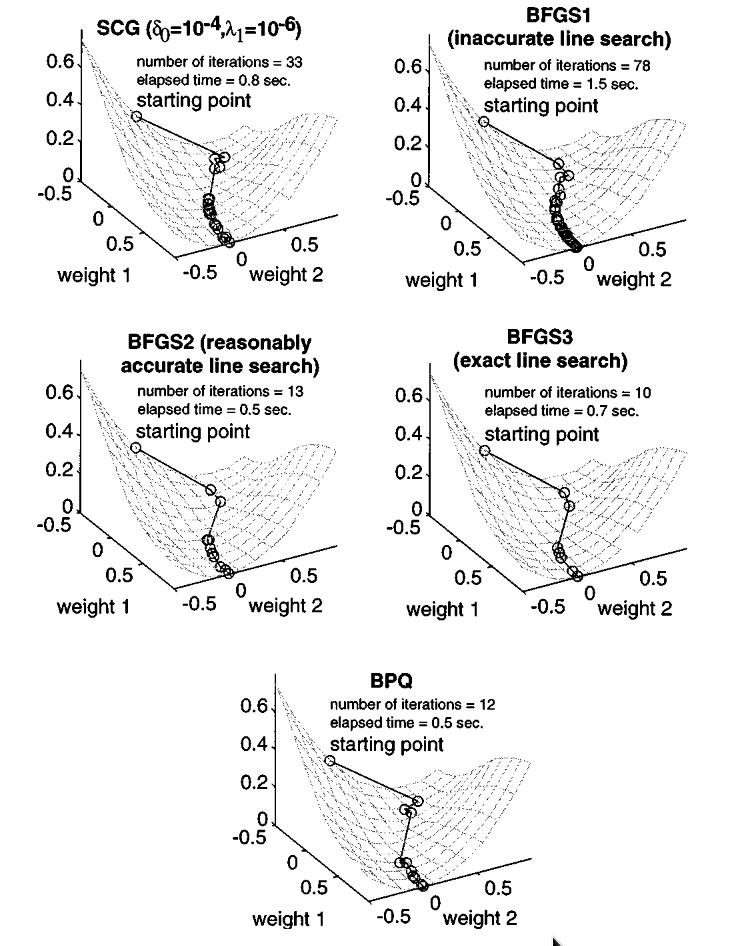
\includegraphics[width=.45\textwidth]{media_tesi/learning_trajectories_of_second_order.jpeg}} \quad
\subfloat[][\emph{Traiettorie algoritmi del secondo ordine}]
{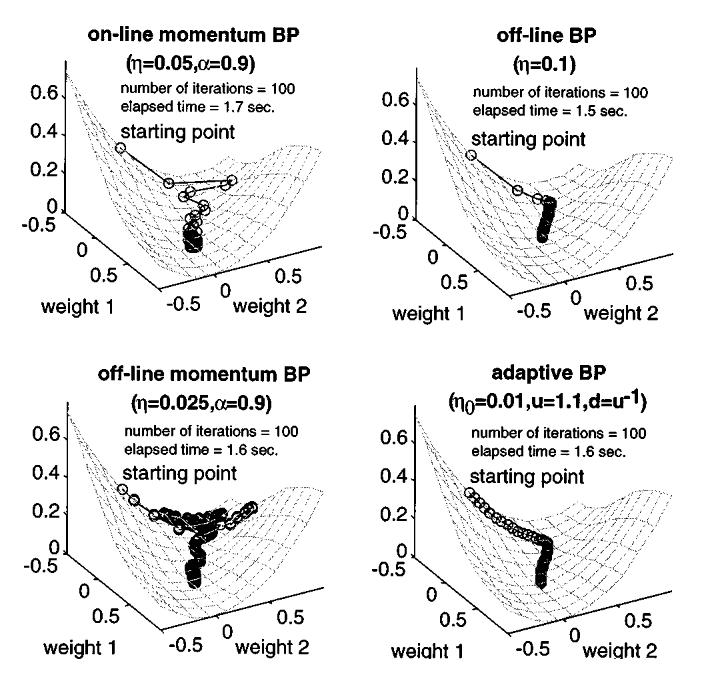
\includegraphics[width=.45\textwidth]{media_tesi/learning_trajectories_of_first_order.jpeg}} \\
\caption{Confronto tra tipologie diverse di algoritmi}
\label{fig:subfig}
\end{figure}


Si può vedere come l'andamento della traiettoria conduca al minimo in numero inferiori di passi utilizzando algoritmi del secondo ordine.

Per velocizzare BP è stato anche introdotto il momento , che ha lo scopo di ridurre le oscillazioni della traiettoria dovute ad una non proficua scelta della lunghezza del passo per le iterazioni e fu proprio nel 1988 che Robert A. Jacobs, propose quattro euristiche per il miglioramento del tasso di convergenza del BP.

Nel 1988 la ricerca aveva già riconosciuto la bontà della procedura BP e si investigavano quegli algoritmi di ricerca dell'ottimo per la funzione di minimo che computassero la discesa del gradiente soltanto localmente (ovvero rimanendo in intorni molto vicini al punto di iterazione). Questo cosidetto \textit{locality constraint} veniva motivato dal fatto che costituiva una buona metafora tecnologica della controparte biologica , le reti neurali, a cui si ispirava e in secondo luogo dall'ipotesi che questi algoritmi \textit{locali} fossero più adatti ad essere processati in parallelo.
Fra le quattro euristiche di Jacobs vi era l'adattamento dei tassi d'apprendimento nel tempo e si spiega che ogni peso della rete dovrebbe avere il proprio tasso d'apprendimento specifico. Le implementazioni di queste euristiche venivano individuate nel \textit{momento} e nella regola d'apprendimento \textit{delta-bar-delta}.
\subsection*{low complexity NNs}
Alcuni altri indirizzi di miglioramento dell'efficacia delle reti sfruttano il BP per modellare delle reti meno complesse (\textit{low complexity}) che possano essere utili a scopi meno sofisticati. Ad esempio, nelle reti convuluzionali, dove il processo di riconoscimento degli oggetti ha luogo, gli algoritmi vengono eseguiti su costese GPU che dissipano grandi quantità di energia e un tale scenario non è adatto a scopi dove il livello di dettaglio nel riconoscere gli oggetti non è così elevato. Applicazioni più popolari e frequenti come il riconoscimento facciale nei dispositivi mobili deve per forza di cose girare in locale sui processori embedded che animano gli smartphone, per questo i ricercatori sfruttano varianti del BP per creare reti convuluzionali a bassa complessità. Queste modellano problemi molto meno \textit{demanding} e possono quindi essere eseguite più velocemente anche sui dispositivi meno prestanti\cite{TSD}.